\documentclass[11pt, a4paper, twoside]{article}

% ─── Font & Encoding ───────────────────────────────────────────────────────────
\usepackage[T1]{fontenc}
\usepackage[utf8]{inputenc}
\usepackage{mathptmx}          % Times New Roman for body and math
\usepackage{microtype}         % Professional microtypography

% ─── Page Layout ───────────────────────────────────────────────────────────────
\usepackage[
  a4paper,
  top=2.5cm, bottom=2.5cm,
  inner=3cm, outer=2.5cm,
  headheight=15pt
]{geometry}
\usepackage{fancyhdr}
\pagestyle{fancy}
\fancyhf{}
\fancyhead[LE,RO]{\small\thepage}
\fancyhead[LO]{\small\nouppercase{\rightmark}}
\fancyhead[RE]{\small\nouppercase{Conversational Graph Memory}}
\renewcommand{\headrulewidth}{0.4pt}

% ─── Mathematics & Algorithms ──────────────────────────────────────────────────
\usepackage{amsmath, amssymb, amsthm}
\usepackage[ruled, vlined, linesnumbered]{algorithm2e}

% ─── Tables ────────────────────────────────────────────────────────────────────
\usepackage{booktabs}
\usepackage{array}
\usepackage{tabularx}
\usepackage{multirow}

% ─── Figures & Diagrams ────────────────────────────────────────────────────────
\usepackage{tikz}
\usetikzlibrary{
  arrows.meta,
  shapes.geometric,
  shapes.misc,
  fit,
  positioning,
  calc,
  decorations.pathreplacing,
  decorations.markings,
  matrix,
  backgrounds
}
\usepackage{graphicx}
\usepackage{float}

% ─── Code Listings ─────────────────────────────────────────────────────────────
\usepackage{listings}
\lstset{
  basicstyle=\small\ttfamily,
  breaklines=true,
  frame=single,
  numbers=left,
  numberstyle=\tiny,
  tabsize=4,
  showstringspaces=false,
  captionpos=b
}

% ─── References & Links ────────────────────────────────────────────────────────
\usepackage[hidelinks]{hyperref}
\usepackage{cleveref}

% ─── Misc ──────────────────────────────────────────────────────────────────────
\usepackage{enumitem}
\usepackage{setspace}
\usepackage{caption}
\usepackage{subcaption}
\usepackage{titlesec}
\usepackage{abstract}
\usepackage{xspace}

% ─── TikZ Styles ───────────────────────────────────────────────────────────────
\tikzset{
  block/.style={
    rectangle, draw, thick,
    minimum width=2.8cm, minimum height=0.9cm,
    align=center, font=\small
  },
  wideblock/.style={
    rectangle, draw, thick,
    minimum width=4.5cm, minimum height=0.9cm,
    align=center, font=\small
  },
  tallblock/.style={
    rectangle, draw, thick,
    minimum width=2.8cm, minimum height=1.4cm,
    align=center, font=\small
  },
  roundblock/.style={
    rectangle, rounded corners=4pt, draw, thick,
    minimum width=2.8cm, minimum height=0.9cm,
    align=center, font=\small
  },
  database/.style={
    cylinder, shape border rotate=90, draw, thick,
    minimum width=2.2cm, minimum height=1.2cm,
    align=center, font=\small, aspect=0.3
  },
  decision/.style={
    diamond, draw, thick,
    minimum width=2.4cm, minimum height=1.1cm,
    align=center, font=\small, inner sep=1pt
  },
  arrow/.style={-{Stealth[scale=1.2]}, thick},
  dasharrow/.style={-{Stealth[scale=1.2]}, thick, dashed},
  bigarrow/.style={-{Stealth[scale=1.5]}, very thick},
  groupbox/.style={
    rectangle, draw, thick, dashed,
    inner sep=8pt, rounded corners=3pt
  }
}

% ─── Theorem Environments ──────────────────────────────────────────────────────
\theoremstyle{definition}
\newtheorem{definition}{Definition}[section]
\newtheorem{remark}{Remark}[section]

% ─── Custom Commands ───────────────────────────────────────────────────────────
\newcommand{\CGM}{\textsc{CGM}\xspace}
\newcommand{\KV}{\textit{KV}\xspace}

% ─── Title ─────────────────────────────────────────────────────────────────────
\title{
  \Large\textbf{Conversational Graph Memory (CGM)}\\[0.5em]
  \large A Semantic Architecture for Replacing Per-Turn KV Caches\\
  in Large Language Model Inference\\[0.5em]
  \normalsize\textit{Technical Specification, Research Motivation, and Execution Roadmap}
}

\author{
  \textit{Conceptual Design by the Originating Author}\\[0.3em]
  \small Documented for Research Development and Implementation Reference
}

\date{\today}

% ═══════════════════════════════════════════════════════════════════════════════
\begin{document}
% ═══════════════════════════════════════════════════════════════════════════════

\maketitle
\thispagestyle{empty}

\begin{abstract}
\noindent
Large language model (LLM) inference at scale is increasingly bottlenecked by the
memory consumed by the Key-Value (KV) cache in multi-turn conversations. For a single
long conversation, this cache may occupy tens of gigabytes of GPU memory, scaling
linearly with the number of tokens exchanged. Existing mitigation strategies---token
eviction, quantization, and low-rank compression---reduce the magnitude of this problem
but preserve the fundamental representation: floating-point attention tensors. This
paper presents \CGM (\textbf{C}onversational \textbf{G}raph \textbf{M}emory), a novel
architecture that changes the representation type entirely. After each conversational
turn completes, \CGM extracts a compact semantic graph of entities, relationships, and
episodic annotations from the conversation text, discards the raw KV cache, and persists
only the graph---reducing inter-turn memory from the gigabyte to the kilobyte scale.
At the start of each subsequent turn, a learned encoder reconstructs a compact set of
KV-compatible vectors from the retrieved graph and injects them directly into the
transformer attention layers, providing the model with semantically distilled context
rather than a verbatim token history. The architecture introduces a closed loop:
$\text{KV} \rightarrow \text{Semantic Graph} \rightarrow \text{KV}$. We describe the
full system design, each architectural component in detail, the theoretical novelty
relative to existing published work, the key research hypotheses that must be validated,
and a staged implementation roadmap accessible to practitioners with varying levels
of ML expertise.
\end{abstract}

\vspace{1em}
\noindent\textbf{Keywords:} KV cache compression, semantic memory, knowledge graph,
multi-turn inference, transformer memory, LLM serving, neural-symbolic architecture,
conversational AI.

\newpage
\tableofcontents
\newpage

% ═══════════════════════════════════════════════════════════════════════════════
\section{Introduction and Motivation}
\label{sec:intro}
% ═══════════════════════════════════════════════════════════════════════════════

\subsection{The Multi-Turn Inference Crisis}

The deployment of large language models in production multi-turn conversation systems
has revealed a fundamental tension between context quality and memory efficiency. Every
token a transformer model processes requires it to compute and store a Key vector and
a Value vector for each of its attention layers and heads. These vectors collectively
constitute the \textbf{Key-Value (KV) cache}. The cache enables the model to attend
over its entire conversational history at each new generation step---but the memory
cost grows without bound as the conversation lengthens.

\medskip

For a model such as LLaMA 3 70B, a single generated token contributes approximately
1 MB to the KV cache across all layers. A conversation of 4,000 tokens therefore
accumulates roughly 4 GB of KV state for a single user session. When the context
window extends to 128,000 tokens---a common target in modern deployments---the KV
cache for a single conversation can exceed 40 GB, more than the model weights
themselves require. Serving a hundred concurrent users under these conditions would
demand KV memory alone in excess of 4 TB.

\medskip

The economic consequence is severe. The AI inference market is projected to reach
\$255 billion by 2030. Major AI labs already report inference costs exceeding training
costs by an order of magnitude. A significant portion of this cost is attributable to
KV cache management, memory bandwidth overhead, and the GPU memory fragmentation
introduced by variable-length conversation histories. Research based on production
conversation datasets (ShareGPT) indicates that approximately 73\% of all inference
traffic is multi-turn, meaning the KV cache problem is the common case, not the edge case.

\subsection{What Existing Solutions Do---and Do Not---Solve}

The research community has produced a number of effective techniques for reducing KV
cache overhead. These include:

\begin{itemize}[leftmargin=*]
  \item \textbf{Token eviction} (SnapKV, StreamingLLM): discards tokens deemed
    low-salience based on accumulated attention weights. Reduces cache size but
    retains the KV tensor format.
  \item \textbf{Quantization} (KVQuant, MixedQ): reduces the bit-width of stored
    KV vectors from 16-bit floats to 8-bit or 4-bit integers. Achieves
    approximately $2\times$--$4\times$ compression within the same format.
  \item \textbf{Low-rank decomposition} (SVDq, xKV): approximates the key
    matrix as a product of lower-dimensional matrices. Computationally expensive;
    performed at prefill time.
  \item \textbf{Semantic chunking} (ChunkKV, SentenceKV): treats
    linguistically coherent chunks rather than individual tokens as the unit of
    compression. Improves quality preservation under eviction.
  \item \textbf{Multi-turn isolation} (FlowKV): preserves compressed KV from past
    turns and compresses only the newly completed turn, preventing re-compression
    of older context.
\end{itemize}

\medskip

Every one of these methods shares a defining characteristic: \textit{the KV cache
remains a KV cache}. The representation type is unchanged. Compression ratios in
practice remain within one to two orders of magnitude of the original size. The
gigabyte-scale storage problem at the inter-turn boundary is mitigated but not
structurally resolved.

\subsection{The Core Insight of This Work}

\CGM is motivated by a simple but radical observation: \textbf{the KV cache is cached
computation, not memory}. It exists because transformers process sequences token by
token and need to avoid redundant attention computation. It is not an intentional
memory architecture---it is a computational artifact. The fact that it has become the
de facto mechanism for conversational context persistence is a consequence of how
transformers were designed, not a principled choice about how AI systems should remember.

\medskip

The core insight is this: what a model needs to continue a conversation coherently is
not the verbatim token history---it is the \textit{meaning} of that history. The
entities that were introduced, the relationships between them, the preferences and goals
expressed by the user, the facts established, the epistemic states held. This meaning
can be represented far more compactly as a structured semantic graph than as a matrix
of floating-point attention vectors.

\medskip

\CGM operationalises this insight by:
\begin{enumerate}[leftmargin=*]
  \item Extracting a semantic graph from each completed conversational turn.
  \item Discarding the raw KV cache for that turn.
  \item Persisting only the graph (kilobytes, not gigabytes).
  \item Reconstructing a compact set of KV-compatible vectors from the graph at
    the start of each subsequent turn.
  \item Injecting those vectors directly into the transformer's attention layers.
\end{enumerate}

This creates the central computational loop of the system:
\begin{align*}
\underbrace{\text{KV Cache}}_{\text{GB scale}}
&\;\longrightarrow\;
\underbrace{\text{Graph Extraction}}_{\text{turn boundary}}
\;\longrightarrow\;
\underbrace{\text{Graph Store}}_{\text{KB scale}}\\[4pt]
&\;\longrightarrow\;
\underbrace{\text{KV Reconstruction}}_{\text{next turn start}}
\;\longrightarrow\;
\underbrace{\text{KV Injection}}_{\text{compact context}}
\end{align*}

% ═══════════════════════════════════════════════════════════════════════════════
\section{System Architecture Overview}
\label{sec:architecture}
% ═══════════════════════════════════════════════════════════════════════════════

\subsection{High-Level Pipeline}

\Cref{fig:pipeline} illustrates the complete \CGM pipeline across two consecutive
conversational turns. At the turn boundary, the system transitions from the standard
transformer inference regime (in which the KV cache accumulates) to the \CGM
compression regime (in which the graph is extracted and the cache discarded).

\begin{figure}[H]
\centering
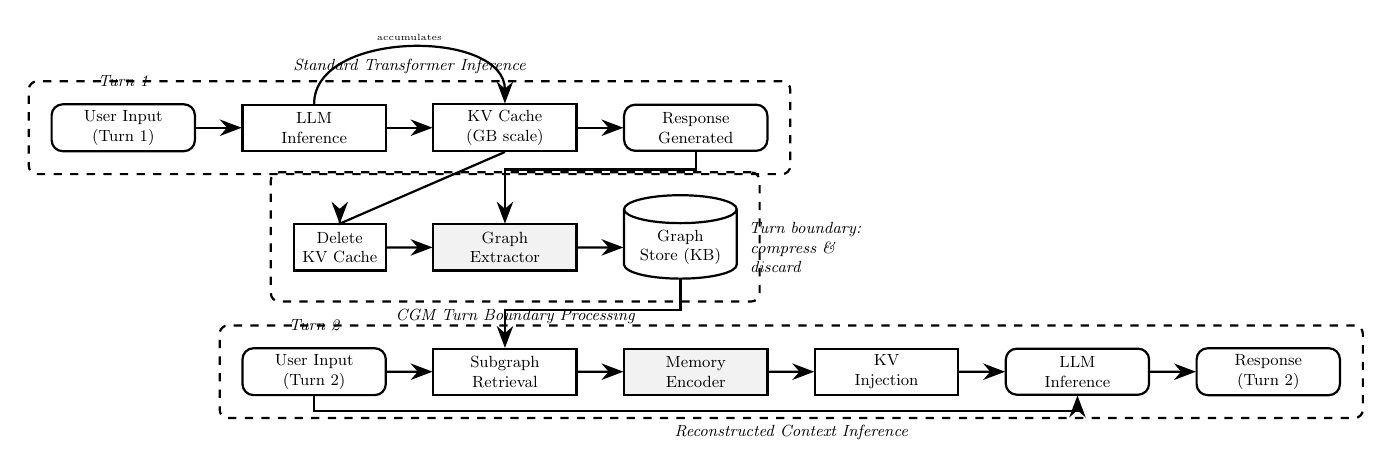
\begin{tikzpicture}[scale=0.65, transform shape, node distance=0.6cm and 0.5cm]

% ── Turn 1 cluster ──────────────────────────────────────────────────────────
\node[roundblock] (user1) {User Input\\(Turn 1)};
\node[block, right=0.9cm of user1] (llm1) {LLM\\Inference};
\node[block, right=0.9cm of llm1] (kvcache) {KV Cache\\(GB scale)};
\node[roundblock, right=0.9cm of kvcache] (resp1) {Response\\Generated};

\draw[arrow] (user1) -- (llm1);
\draw[arrow] (llm1) -- (kvcache);
\draw[arrow] (kvcache) -- (resp1);
\draw[arrow] (llm1.north) to[out=90,in=90] node[above,font=\tiny]{accumulates} (kvcache.north);

% Turn 1 label
\node[above=0.2cm of user1, font=\small\itshape] {Turn 1};

% ── Turn boundary ────────────────────────────────────────────────────────────
\node[block, below=1.4cm of kvcache, fill=black!5] (extractor)
  {Graph\\Extractor};
\node[database, right=0.9cm of extractor] (graphstore)
  {Graph\\Store (KB)};
\node[block, below=0.6cm of kvcache, draw=none, font=\small\itshape]
  (boundary) {};

% Delete symbol
\node[block, left=0.9cm of extractor, draw, thick, minimum width=1.8cm,
      minimum height=0.9cm, font=\small] (del) {Delete\\KV Cache};

\draw[arrow] (resp1.south) -- ++(0,-0.35) -| (extractor.north);
\draw[arrow] (kvcache.south) -- (del.north |- extractor.north) -- (del.north);
\draw[arrow] (del) -- (extractor);
\draw[arrow] (extractor) -- (graphstore);

% Boundary annotation
\node[right=0.15cm of graphstore, font=\small\itshape, text width=2.2cm]
  {\textit{Turn boundary:\\ compress \& discard}};

% ── Turn 2 cluster ──────────────────────────────────────────────────────────
\node[block, below=1.5cm of extractor] (retriever)
  {Subgraph\\Retrieval};
\node[block, right=0.9cm of retriever, fill=black!5] (encoder)
  {Memory\\Encoder};
\node[block, right=0.9cm of encoder] (inject)
  {KV\\Injection};
\node[roundblock, right=0.9cm of inject] (llm2)
  {LLM\\Inference};
\node[roundblock, right=0.9cm of llm2] (resp2)
  {Response\\(Turn 2)};

\node[roundblock, left=0.9cm of retriever] (user2) {User Input\\(Turn 2)};

\draw[arrow] (user2) -- (retriever);
\draw[arrow] (graphstore.south) -- ++(0,-0.6) -| (retriever.north);
\draw[arrow] (retriever) -- (encoder);
\draw[arrow] (encoder) -- (inject);
\draw[arrow] (inject) -- (llm2);
\draw[arrow] (llm2) -- (resp2);
\draw[arrow] (user2.south) -- ++(0,-0.3) -| (llm2.south);

% Turn 2 label
\node[above=0.2cm of user2, font=\small\itshape] {Turn 2};

% ── Bounding boxes ───────────────────────────────────────────────────────────
\begin{scope}[on background layer]
  \node[groupbox, fit=(user1)(llm1)(kvcache)(resp1),
        label={[font=\small\itshape]above:Standard Transformer Inference}] {};
  \node[groupbox, fit=(del)(extractor)(graphstore),
        label={[font=\small\itshape]below:CGM Turn Boundary Processing}] {};
  \node[groupbox, fit=(user2)(retriever)(encoder)(inject)(llm2)(resp2),
        label={[font=\small\itshape]below:Reconstructed Context Inference}] {};
\end{scope}

\end{tikzpicture}
\caption{The \CGM pipeline spanning two consecutive conversational turns.
At the turn boundary, the KV cache is extracted into a semantic graph, the raw
cache is deleted, and the graph is persisted in kilobyte-scale storage. On the
next turn, a subgraph is retrieved, encoded into compact KV vectors, and injected
into the transformer's attention mechanism.}
\label{fig:pipeline}
\end{figure}

\subsection{Component Decomposition}

\CGM comprises seven functional components, each responsible for a well-defined
stage in the pipeline. \Cref{tab:components} provides a summary; subsequent
sections describe each in full detail.

\begin{table}[H]
\centering
\caption{Summary of \CGM architectural components.}
\label{tab:components}
\begin{tabularx}{\textwidth}{@{}llX@{}}
\toprule
\textbf{Component} & \textbf{Stage} & \textbf{Responsibility} \\
\midrule
Graph Extractor & Turn boundary & Converts conversation text to semantic triples,
  embeddings, and episodic annotations. \\
Hybrid Memory Object & Turn boundary & Structured container combining graph,
  embeddings, summaries, and temporal metadata. \\
Graph Store & Persistence & Lightweight key-value storage of per-conversation
  graphs at KB scale. \\
Subgraph Retriever & Turn start & Identifies which portions of the stored graph
  are relevant to the incoming query. \\
Memory Encoder Network & Turn start & Learnable encoder that converts retrieved
  graph representations into transformer-compatible KV vectors. \\
KV Injector & Turn start & Inserts encoded memory vectors into the attention
  layers of the frozen LLM. \\
Fidelity Evaluator & Offline & Measures semantic preservation quality across
  compression-reconstruction cycles. \\
\bottomrule
\end{tabularx}
\end{table}

% ═══════════════════════════════════════════════════════════════════════════════
\section{Component Specifications}
\label{sec:components}
% ═══════════════════════════════════════════════════════════════════════════════

\subsection{Component 1: The Graph Extractor}
\label{sec:extractor}

The Graph Extractor operates on the \textit{text} of a completed conversational turn,
not on the raw KV vectors. This distinction is critical. KV vectors are distributed
floating-point tensors with no interpretable symbolic structure---entity names and
semantic relations cannot be read out of them directly. The conversation text, however,
is always available as it generated the KV cache and is the natural source for semantic
extraction.

\medskip

The extractor executes three sub-processes in sequence:

\begin{enumerate}[leftmargin=*]
  \item \textbf{Named Entity Recognition (NER):} Identifies entities of relevant
    types (persons, organisations, concepts, artefacts, locations, programming
    constructs, and so on) present in the turn. Assigns each entity a unique
    identifier within the conversation graph.
  \item \textbf{Relation Extraction (RE):} Identifies typed directed relations
    between entity pairs. Outputs semantic triples of the form
    $\langle \textit{subject}, \textit{predicate}, \textit{object} \rangle$.
    Example: $\langle \textsc{User}, \textit{prefers}, \textsc{Python} \rangle$.
  \item \textbf{Coreference Resolution:} Resolves pronouns and nominal anaphors
    to their referent entities, ensuring that ``it'' and ``the system'' are
    linked to the correct entity nodes across the graph.
\end{enumerate}

The extractor can be implemented at three levels of sophistication, chosen
according to available compute and required fidelity:

\begin{description}[leftmargin=*, style=nextline]
  \item[Level 1 (Prompt-based):] Instruct a small language model (e.g.,
    a 1B--3B parameter instruction-tuned model) to extract triples from the
    turn text in structured JSON format. No training required. Slower but
    immediately deployable.
  \item[Level 2 (Pipeline-based):] Use a classical NLP pipeline such as
    spaCy with a fine-tuned NER and RE model. Fast, deterministic,
    well-understood.
  \item[Level 3 (Specialised):] Fine-tune a dedicated extraction model on
    conversational triple extraction data. Highest quality; requires training.
\end{description}

\subsubsection{Handling Nuance and Non-Factual Content}

A pure triple representation captures facts but loses epistemic stance, emotional
tone, and hedged language. The sentence \textit{``I am not entirely sure I trust
that approach''} does not reduce cleanly to a triple. To address this, the Graph
Extractor additionally produces:

\begin{itemize}[leftmargin=*]
  \item \textbf{Semantic embeddings:} A dense vector encoding of each sentence,
    preserving latent tonal and semantic information not captured by triples.
  \item \textbf{Uncertainty scores:} Per-claim confidence values extracted from
    hedging language (\textit{``maybe''}, \textit{``I think''}, etc.).
  \item \textbf{Conversation summary:} A 2--4 sentence abstractive summary of
    the turn, preserving narrative and stylistic context.
\end{itemize}

\subsection{Component 2: The Hybrid Memory Object}
\label{sec:hybridobject}

The raw output of the extractor is consolidated into a structured Hybrid Memory
Object (HMO) for each completed turn. The HMO is the atomic unit of storage in
the \CGM graph store. Its schema is as follows:

\begin{lstlisting}[language=Python, caption={Hybrid Memory Object schema (Python
dataclass representation).}]
@dataclass
class HybridMemoryObject:
    turn_id: int
    timestamp: float

    # Symbolic tier: structured semantic triples
    triples: List[Triple]           # (subject, predicate, object)

    # Latent tier: dense representations
    sentence_embeddings: np.ndarray # shape: (n_sentences, d_embed)
    style_embedding: np.ndarray     # shape: (d_embed,)
    conversation_embedding: np.ndarray  # shape: (d_embed,)

    # Summary tier: natural language distillation
    summary: str                    # 2-4 sentence abstractive summary

    # Temporal tier: episodic annotations
    episodic_events: List[EpisodicEvent]
    # e.g. {"event": "opinion_change",
    #        "from": "Rust is hard",
    #        "to": "Rust is interesting",
    #        "confidence": 0.91}

    # Uncertainty tier
    uncertainty_scores: Dict[str, float]  # claim_id -> confidence
\end{lstlisting}

This multi-tier design ensures that no single type of information---factual,
latent, narrative, temporal, or epistemic---is discarded at extraction time.
The encoder downstream selects which tiers to use based on the query context.

The estimated storage cost of a typical HMO for a 10-exchange turn (approximately
500--800 tokens) is shown in \Cref{tab:storage}.

\begin{table}[H]
\centering
\caption{Estimated storage footprint per turn under standard conversation conditions.}
\label{tab:storage}
\begin{tabular}{@{}lrr@{}}
\toprule
\textbf{Representation} & \textbf{Typical Size} & \textbf{Notes} \\
\midrule
Raw KV Cache (LLaMA 3 70B) & $\sim$4,000 MB & At 4,000 tokens \\
KV after quantization (8-bit) & $\sim$500--1,000 MB & Existing best practice \\
KV after token eviction (10\%) & $\sim$400 MB & SnapKV-class methods \\
\CGM Semantic Triples (JSON) & $\sim$15--40 KB & 60--120 triples \\
\CGM Embeddings & $\sim$50--80 KB & 768-dim float32 per sentence \\
\CGM Summary (text) & $\sim$1--2 KB & 2--4 sentences \\
\CGM Episodic Annotations & $\sim$5--10 KB & Per turn \\
\textbf{\CGM Total (HMO)} & $\sim$\textbf{70--135 KB} & \textbf{Full hybrid object} \\
\bottomrule
\end{tabular}
\end{table}

The effective compression ratio between the raw KV cache and the \CGM HMO is
approximately $\mathbf{30\times}$--$\mathbf{60\times}$ on a byte basis. More
importantly, this ratio does not represent lossy compression of the same
information---it represents \textit{substitution} of KV geometry with semantic
content. The meaningful question is therefore not the compression ratio but the
\textit{semantic fidelity} of the substitution, which is addressed in
\Cref{sec:fidelity}.

\subsection{Component 3: The Graph Store}
\label{sec:store}

The Graph Store is the persistence layer of \CGM. It maintains a per-conversation
directed multigraph $G = (V, E, A)$ where:

\begin{itemize}[leftmargin=*]
  \item $V$ is the set of entity nodes, each annotated with type and frequency
    information.
  \item $E \subseteq V \times V$ is the set of directed edges, each labelled
    with a relation type and a confidence score.
  \item $A$ is the set of HMOs, one per completed turn, associated with the
    relevant subgraph for that turn.
\end{itemize}

Entity merging across turns is handled by a coreference module that checks whether
newly extracted entities map to existing nodes (by name normalisation and embedding
similarity). This ensures that references to the same entity across turns are
unified in the graph rather than duplicated.

The store can be implemented as a lightweight embedded graph database (e.g.,
NetworkX for prototyping, or Neo4j / DuckDB for production) or as a plain JSON
file for initial experimentation. For a conversation of 20 turns, the total store
size is typically 1--3 MB---small enough to reside in RAM or be retrieved from disk
in milliseconds.

\subsection{Component 4: The Subgraph Retriever}
\label{sec:retriever}

When a new user message arrives at the start of Turn $n+1$, the Subgraph Retriever
identifies which portions of the stored graph $G$ are relevant to answering it.
Retrieving the entire graph is inefficient and may overload the downstream encoder
with irrelevant information. The retriever performs a multi-signal scoring procedure.

\medskip

Let $q$ denote the query embedding of the incoming message. For each node $v \in V$
and each HMO $a_t$ from turn $t$, the retrieval score is:

\[
s(v, a_t) = \alpha \cdot \text{sim}(q, e_v)
           + \beta \cdot \text{sim}(q, e_{a_t})
           + \gamma \cdot r(t)
           + \delta \cdot w(v)
\]

where:
\begin{itemize}[leftmargin=*, itemsep=2pt]
  \item $e_v$ is the embedding of entity node $v$.
  \item $e_{a_t}$ is the conversation embedding of HMO $a_t$.
  \item $r(t) = \exp(-\lambda (n - t))$ is a recency decay over turn distance.
  \item $w(v)$ is the accumulated attention-weight proxy for node $v$ (how often
    the entity has appeared across turns).
  \item $\alpha, \beta, \gamma, \delta$ are tunable weighting coefficients.
\end{itemize}

The retriever returns the top-$k$ scoring nodes along with their incident edges
and associated HMO tiers. The value of $k$ is bounded to prevent context overload
at the encoder stage. A typical value is $k = 40$--$80$ triples.

\Cref{fig:retriever} illustrates the retrieval process schematically.

\begin{figure}[H]
\centering
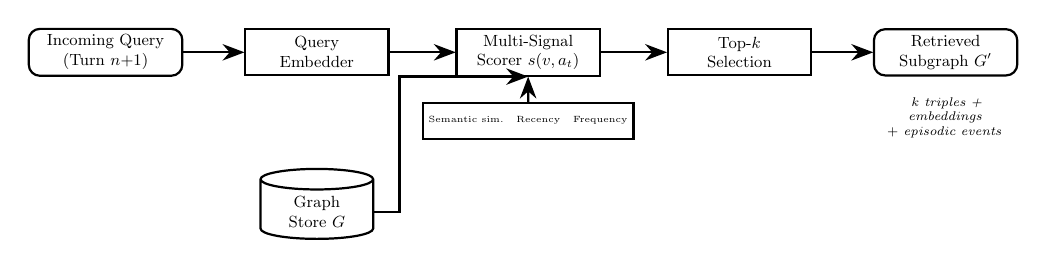
\begin{tikzpicture}[scale=0.65, transform shape, node distance=0.7cm and 0.9cm]

% Query
\node[roundblock, minimum width=3cm] (query) {Incoming Query\\(Turn $n$+1)};
\node[block, right=1.2cm of query] (qembed) {Query\\Embedder};
\draw[arrow] (query) -- (qembed);

% Graph store
\node[database, below=1.8cm of qembed] (gstore) {Graph\\Store $G$};

% Scorer
\node[block, right=1.3cm of qembed] (scorer) {Multi-Signal\\Scorer $s(v,a_t)$};
\draw[arrow] (qembed) -- (scorer);
\draw[arrow] (gstore.east) -- ++(0.5,0) |- (scorer.south);

% Signals feeding scorer
\node[block, below=0.5cm of scorer, minimum width=2.2cm, font=\tiny,
      minimum height=0.7cm] (signals)
  {Semantic sim.~~~Recency~~~Frequency};
\draw[arrow] (signals) -- (scorer);

% Top-k
\node[block, right=1.3cm of scorer] (topk) {Top-$k$\\Selection};
\draw[arrow] (scorer) -- (topk);

% Output subgraph
\node[roundblock, right=1.2cm of topk] (subgraph) {Retrieved\\Subgraph $G'$};
\draw[arrow] (topk) -- (subgraph);

% Annotation
\node[below=0.3cm of subgraph, font=\scriptsize\itshape, text width=2.8cm,
      text centered]
  {$k$ triples + embeddings\\$+$ episodic events};

\end{tikzpicture}
\caption{Subgraph retrieval procedure at the start of Turn $n+1$. The incoming
query is embedded and scored against all nodes and HMOs in the graph store using
a multi-signal function combining semantic similarity, recency, and entity frequency.
The top-$k$ results form the retrieved subgraph passed to the Memory Encoder.}
\label{fig:retriever}
\end{figure}

\subsection{Component 5: The Memory Encoder Network}
\label{sec:encoder}

The Memory Encoder Network (MEN) is the most technically novel and challenging
component of \CGM. Its function is to convert the retrieved subgraph $G'$---a
heterogeneous collection of triples, embeddings, summaries, and episodic
annotations---into a small set of transformer-compatible KV vectors that can be
injected into the LLM's attention layers.

\medskip

This component draws on the architecture of KBLAM (Knowledge Base-Augmented Language
Models, ICLR 2025), which demonstrated that knowledge triples can be encoded into
key-value vector pairs using a pretrained sentence encoder followed by learnable
linear adapter layers, and injected into LLM attention through a rectangular
attention mechanism. The critical distinction between KBLAM and \CGM is the
\textit{source} of the knowledge base:

\begin{itemize}[leftmargin=*]
  \item KBLAM operates on \textit{static, pre-built external knowledge bases}
    (e.g., Wikidata, company wikis). The KB is fixed at deployment time.
  \item \CGM operates on a \textit{dynamic, per-conversation graph} built live
    from the conversation itself. The KB changes every turn.
\end{itemize}

This distribution shift means the MEN cannot be used off-the-shelf from KBLAM
and requires fine-tuning or retraining on conversational data. The architecture
is as follows.

\subsubsection{Encoder Architecture}

For each triple $t_i = \langle s_i, p_i, o_i \rangle$ in the retrieved subgraph,
the encoder constructs an input representation:

\[
x_i = [\,\text{enc}(s_i \,||\, p_i)\,;\;\text{enc}(o_i)\,]
\]

where $\text{enc}(\cdot)$ is a pretrained sentence encoder (e.g., a frozen
Sentence-BERT model) and $[\,;\,]$ denotes concatenation. For each HMO embedding
tier, the conversation embedding $e_{a_t}$ is appended as an additional input token.

A pair of learnable linear adapter layers $W_K$ and $W_V$ project this input
representation into the key and value spaces of the target LLM:

\[
k_i = W_K \cdot x_i, \qquad v_i = W_V \cdot x_i
\]

These synthetic KV pairs are the outputs of the encoder. For a retrieved subgraph
of 60 triples, the encoder produces 60 KV pairs---a small, fixed-size set of vectors
regardless of the original conversation length.

\subsubsection{Training the Memory Encoder}

The MEN is trained with the LLM frozen. The training objective is to minimise the
cross-entropy loss between:
\begin{itemize}[leftmargin=*]
  \item Responses generated by the LLM when given full KV cache context (the target).
  \item Responses generated by the LLM when given only the injected synthetic KV
    vectors from the MEN (the output to be optimised).
\end{itemize}

This requires paired training data of the form:
\[
\mathcal{D} = \{(\text{conversation}_i,\;\text{graph}_i,\;\text{full-KV response}_i)\}
\]

Such a dataset does not yet exist publicly and must be constructed. Construction
procedure is described in \Cref{sec:phase2}.

\begin{figure}[H]
\centering
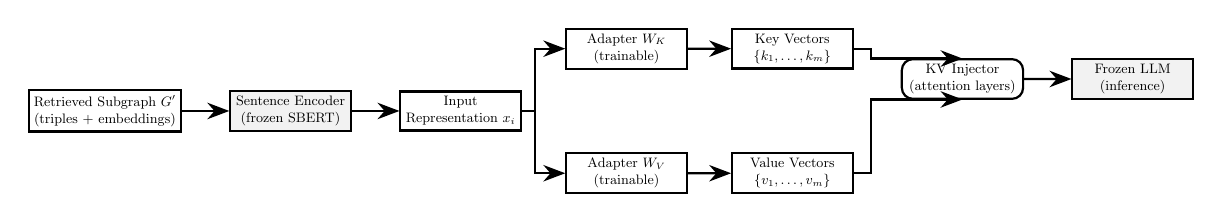
\begin{tikzpicture}[scale=0.55, transform shape, node distance=0.6cm and 0.9cm]

% Input
\node[block, minimum width=3.5cm] (subgraph) {Retrieved Subgraph $G'$\\(triples + embeddings)};

% Sentence encoder
\node[block, right=1.1cm of subgraph, fill=black!5] (sentenc)
  {Sentence Encoder\\(frozen SBERT)};
\draw[arrow] (subgraph) -- (sentenc);

% Representation x_i
\node[block, right=1.1cm of sentenc] (xi) {Input\\Representation $x_i$};
\draw[arrow] (sentenc) -- (xi);

% Adapters
\node[block, above right=0.5cm and 1.0cm of xi] (wk)
  {Adapter $W_K$\\(trainable)};
\node[block, below right=0.5cm and 1.0cm of xi] (wv)
  {Adapter $W_V$\\(trainable)};
\draw[arrow] (xi.east) -- ++(0.3,0) |- (wk.west);
\draw[arrow] (xi.east) -- ++(0.3,0) |- (wv.west);

% Output KV pairs
\node[block, right=1.0cm of wk] (kout) {Key Vectors\\$\{k_1,\ldots,k_m\}$};
\node[block, right=1.0cm of wv] (vout) {Value Vectors\\$\{v_1,\ldots,v_m\}$};
\draw[arrow] (wk) -- (kout);
\draw[arrow] (wv) -- (vout);

% Arrow to injector
\node[roundblock, right=1.1cm of kout, yshift=-0.7cm] (injector)
  {KV Injector\\(attention layers)};
\draw[arrow] (kout.east) -- ++(0.4,0) |- (injector.north);
\draw[arrow] (vout.east) -- ++(0.4,0) |- (injector.south);

% Frozen LLM
\node[block, right=1.1cm of injector, fill=black!5] (llm)
  {Frozen LLM\\(inference)};
\draw[arrow] (injector) -- (llm);

\end{tikzpicture}
\caption{Memory Encoder Network (MEN) architecture. The retrieved subgraph is
processed by a frozen sentence encoder into input representations $x_i$. Trainable
linear adapters $W_K$ and $W_V$ project these into synthetic key and value vectors
which are injected into the frozen LLM's attention layers via the KV Injector.}
\label{fig:encoder}
\end{figure}

\subsection{Component 6: The KV Injector}
\label{sec:injector}

The KV Injector places the synthetic KV vectors produced by the MEN into the
attention computation of the LLM at inference time. Concretely, for each
transformer layer $\ell$, the standard self-attention computation is:

\[
\text{Attn}^\ell(Q, K, V) = \text{softmax}\!\left(\frac{Q K^\top}{\sqrt{d_k}}\right) V
\]

The KV Injector prepends the synthetic vectors to the existing key and value
sequences:

\[
\hat{K}^\ell = [\,K_{\text{mem}}^\ell\,;\;K_{\text{curr}}^\ell\,],
\qquad
\hat{V}^\ell = [\,V_{\text{mem}}^\ell\,;\;V_{\text{curr}}^\ell\,]
\]

where $K_{\text{mem}}^\ell, V_{\text{mem}}^\ell$ are the encoded memory vectors
for layer $\ell$ and $K_{\text{curr}}^\ell, V_{\text{curr}}^\ell$ are the
keys and values from the current turn's tokens. The modified attention is:

\[
\text{Attn}^\ell(Q, \hat{K}, \hat{V}) = \text{softmax}\!\left(\frac{Q \hat{K}^\top}{\sqrt{d_k}}\right) \hat{V}
\]

This is the rectangular attention mechanism described in KBLAM. The model attends
over both its current turn context and the injected memory simultaneously. The
number of injected vectors ($m = $ number of encoded triples) is small relative
to the current turn context, so the computational overhead is proportional to
the graph size, not the original conversation history.

\subsection{Component 7: The Fidelity Evaluator}
\label{sec:fidelity}

The Fidelity Evaluator is an offline evaluation harness used during development
and research to measure how well the \CGM reconstruction cycle preserves the
information that matters for downstream task performance. It is not a runtime
component.

\medskip

The evaluator measures three independent dimensions of fidelity:

\begin{description}[leftmargin=*, style=nextline]
  \item[Factual fidelity $F_f$:] Given a set of factual questions $Q_F$ whose
    answers were established in Turn 1, what proportion does the model answer
    correctly in Turn 2 when using \CGM context versus full KV cache context?
    \[F_f = \frac{|\{q \in Q_F : \text{ans}_{\CGM}(q) = \text{ans}_{KV}(q)\}|}{|Q_F|}\]
  \item[Preference fidelity $F_p$:] Given user preferences expressed in Turn 1
    (programming language choices, formatting preferences, stated goals), what
    proportion are correctly reflected in Turn 2 responses?
  \item[Reasoning fidelity $F_r$:] On multi-hop questions that require chaining
    two or more facts established in Turn 1, what proportion does the model answer
    correctly?
\end{description}

The target threshold for all three dimensions---what the system must achieve to
be considered a viable replacement for full KV cache---is $F_f, F_p, F_r \geq 0.85$
on task types of interest. This threshold is domain-dependent and should be
calibrated per deployment workload.

% ═══════════════════════════════════════════════════════════════════════════════
\section{Theoretical Novelty and Related Work}
\label{sec:novelty}
% ═══════════════════════════════════════════════════════════════════════════════

\subsection{Positioning in the Literature}

\CGM occupies a position that is distinct from all major existing research directions
in LLM memory and context management. \Cref{tab:novelty} provides a structured
comparison.

\begin{table}[H]
\centering
\caption{Positioning of \CGM relative to existing published work.}
\label{tab:novelty}
\renewcommand{\arraystretch}{1.3}
\begin{tabularx}{\textwidth}{@{}lXX@{}}
\toprule
\textbf{System / Method} & \textbf{What it does} & \textbf{Key difference from \CGM} \\
\midrule
SnapKV, StreamingLLM & Evicts low-salience tokens from KV cache & Stays in KV
  format; does not change representation type \\
ChunkKV, SentenceKV & Semantic chunking as compression unit & Still KV-format
  compression; no cross-turn replacement \\
FlowKV & Multi-turn KV isolation and compression & Evicts within KV format;
  does not discard and replace with graph \\
Infini-Attention & Compressive memory matrix alongside local attention & Fixed-size
  linear-attention summary matrix, not semantic graph; not per-conversation \\
KBLAM & Graph-to-KV injection for static KBs & Source is static external KB,
  not a live per-conversation dynamic graph \\
SR-KI, ConceptFormer & Triple-to-KV encoding & Same limitation as KBLAM; static
  external sources only \\
Zep, SGMem & Agent-layer knowledge graph memory & External retrieval layer above
  the model; does not replace KV; requires text token injection \\
MemGPT & Hierarchical in-context and external memory & Operates at the agent and
  token level; no KV replacement \\
\textbf{\CGM (this work)} & \textbf{Live per-conversation KV$\to$graph$\to$KV cycle} &
  \textbf{First closed-loop system using conversation's own text as dynamic graph
  source for KV reconstruction} \\
\bottomrule
\end{tabularx}
\end{table}

\subsection{The Genuine Novelty Claim}

The novelty of \CGM rests on the \textbf{closed-loop architecture}: the conversation
generates its own graph, the graph replaces the KV cache, and the graph reconstructs
the KV context for the next turn. No published system treats the live conversation
text as the source for dynamic graph construction that then feeds a KV injection
mechanism. KBLAM and SR-KI demonstrate that the injection half of this loop
is feasible; \CGM's contribution is the extraction half and the connection between
them as a unified architecture.

\subsection{The Strongest Technical Concern: Distribution Shift}

The most significant open technical risk is what may be called the
\textit{distribution shift problem}. Standard LLMs are trained exclusively on
sequential token continuation. Their attention weights were learned assuming that
the key and value vectors at each position correspond to actual input tokens
processed in sequence. Synthetic KV vectors produced by the MEN are not actual
token representations---they are learned projections of symbolic triples. The
model has never seen this type of input during pretraining.

\medskip

Three possible outcomes are possible:
\begin{enumerate}[leftmargin=*]
  \item \textbf{Graceful degradation:} The MEN learns to produce vectors that
    are close enough in the attention geometry to real KV vectors that the model
    uses them productively without fine-tuning. This is the best case and the
    hypothesis that KBLAM's success on static KBs provides some evidence for.
  \item \textbf{Adapter-resolved degradation:} The base model cannot use
    synthetic vectors well, but fine-tuning small LoRA adapters in the frozen LLM
    resolves the distribution shift without full retraining.
  \item \textbf{Architecture-level failure:} The gap between symbolic graph
    encodings and learned token KV geometry is too large to bridge without
    retraining the full model. This would require the approach to pivot to a
    text-injection model (agent-layer, not KV-layer).
\end{enumerate}

The fidelity experiment in Phase 1 (\Cref{sec:phase1}) is designed to distinguish
between these three outcomes before significant engineering effort is committed
to the production architecture.

% ═══════════════════════════════════════════════════════════════════════════════
\section{Hierarchical Memory Architecture}
\label{sec:hierarchy}
% ═══════════════════════════════════════════════════════════════════════════════

A critical design principle in \CGM is that not all context should be compressed
equally, and not all of it should be compressed immediately. The system implements
a four-tier memory hierarchy modelled after operating system page management, where
data migrates from faster and larger representations to slower and smaller ones
as it ages.

\begin{figure}[H]
\centering
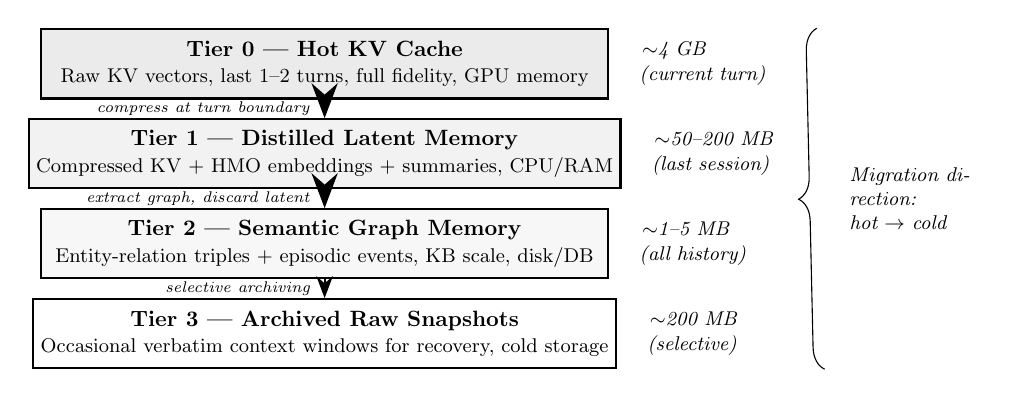
\begin{tikzpicture}[scale=0.8, transform shape, node distance=0.5cm]

\def\tw{9cm}

% Tier 0
\node[rectangle, draw, thick, minimum width=\tw, minimum height=1.1cm,
      align=center, fill=black!8] (t0)
  {\textbf{Tier 0 --- Hot KV Cache}\\
   \small Raw KV vectors, last 1--2 turns, full fidelity, GPU memory};

% Tier 1
\node[rectangle, draw, thick, minimum width=\tw, minimum height=1.1cm,
      align=center, fill=black!5, below=0.3cm of t0] (t1)
  {\textbf{Tier 1 --- Distilled Latent Memory}\\
   \small Compressed KV + HMO embeddings + summaries, CPU/RAM};

% Tier 2
\node[rectangle, draw, thick, minimum width=\tw, minimum height=1.1cm,
      align=center, fill=black!3, below=0.3cm of t1] (t2)
  {\textbf{Tier 2 --- Semantic Graph Memory}\\
   \small Entity-relation triples + episodic events, KB scale, disk/DB};

% Tier 3
\node[rectangle, draw, thick, minimum width=\tw, minimum height=1.1cm,
      align=center, below=0.3cm of t2] (t3)
  {\textbf{Tier 3 --- Archived Raw Snapshots}\\
   \small Occasional verbatim context windows for recovery, cold storage};

% Annotations on right
\node[right=0.4cm of t0, font=\small\itshape, text width=2.5cm] {$\sim$4 GB\\(current turn)};
\node[right=0.4cm of t1, font=\small\itshape, text width=2.5cm] {$\sim$50--200 MB\\(last session)};
\node[right=0.4cm of t2, font=\small\itshape, text width=2.5cm] {$\sim$1--5 MB\\(all history)};
\node[right=0.4cm of t3, font=\small\itshape, text width=2.5cm] {$\sim$200 MB\\(selective)};

% Arrows showing migration
\draw[bigarrow] (t0.south) -- node[left=0.1cm, font=\scriptsize\itshape] {compress at turn boundary} (t1.north);
\draw[bigarrow] (t1.south) -- node[left=0.1cm, font=\scriptsize\itshape] {extract graph, discard latent} (t2.north);
\draw[dasharrow] (t2.south) -- node[left=0.1cm, font=\scriptsize\itshape] {selective archiving} (t3.north);

% Brace
\draw[decorate, decoration={brace, amplitude=8pt, mirror}]
  ([xshift=3.3cm]t0.north east) -- ([xshift=3.3cm]t3.south east)
  node[midway, right=10pt, font=\small\itshape, text width=2.2cm]
  {Migration direction:\\ hot $\to$ cold};

\end{tikzpicture}
\caption{Four-tier hierarchical memory architecture of \CGM. Context migrates
from Tier 0 (hot, full-fidelity KV on GPU) through Tier 1 (compressed latent
memory in CPU RAM) to Tier 2 (semantic graph on disk). Tier 3 provides optional
archival snapshots for recovery from retrieval failures.}
\label{fig:hierarchy}
\end{figure}

The rationale for Tier 3 (archived raw snapshots) is robustness. The retriever
and encoder may occasionally fail to surface critical context that was established
in an early turn but not retrieved. Sparse verbatim snapshots---one per every five
turns, for example---provide a recovery path. When the model signals low-confidence
output or the user corrects a factual error, the system can fall back to the nearest
archived snapshot.

% ═══════════════════════════════════════════════════════════════════════════════
\section{Research Hypotheses}
\label{sec:hypotheses}
% ═══════════════════════════════════════════════════════════════════════════════

Before the full system is engineered, three primary research hypotheses must be
validated through experiment. These are stated formally to enable rigorous testing.

\medskip

\begin{description}[leftmargin=*, style=nextline]
  \item[\textbf{H1 --- Factual Fidelity Hypothesis}:] A model provided with
    graph-reconstructed KV context (via \CGM) achieves factual recall accuracy
    $F_f \geq 0.85$ relative to a full-KV-cache baseline on factual multi-turn
    benchmarks (LoCoMo, LongMemEval).
    
  \item[\textbf{H2 --- Reasoning Preservation Hypothesis}:] A model provided with
    \CGM context achieves multi-hop reasoning accuracy $F_r \geq 0.80$ relative to
    full-KV baseline on benchmarks requiring chain-of-fact inference across turns.
    
  \item[\textbf{H3 --- Compression Viability Hypothesis}:] At the fidelity levels
    established by H1 and H2, the \CGM architecture achieves a mean inter-turn
    storage reduction of at least $100\times$ relative to the uncompressed KV cache.
\end{description}

H1 and H2 must be confirmed before any production-oriented systems engineering begins.
H3 is expected to hold trivially if the extraction and storage components are
implemented as specified, and is stated primarily for the purpose of formal
benchmarking.

% ═══════════════════════════════════════════════════════════════════════════════
\section{Implementation Roadmap}
\label{sec:roadmap}
% ═══════════════════════════════════════════════════════════════════════════════

The implementation is divided into four phases, structured so that each phase
produces a standalone result and de-risks the subsequent phase. A practitioner
with limited ML background can complete Phase 1 with only Python and PyTorch
familiarity. Later phases progressively require deeper ML expertise.

\subsection{Phase 1: Fidelity Validation (Weeks 1--6)}
\label{sec:phase1}

\textbf{Objective:} Determine whether semantic graph context preserves enough
information for coherent multi-turn conversation without any custom training.
This phase tests Hypothesis H1.

\medskip

\textbf{Setup:}
\begin{itemize}[leftmargin=*]
  \item Model: LLaMA 3.2 1B (runs on a consumer laptop or Google Colab).
  \item Task type: Factual multi-turn conversation (coding assistant scenario:
    user establishes preferences and code context over 5 turns, then continues
    for 5 more turns).
  \item Context replacement: After turn 5, replace the KV cache with a
    structured text prompt containing extracted triples (no custom encoder,
    no KV injection---plain text only).
\end{itemize}

\textbf{Experiment procedure:}
\begin{enumerate}[leftmargin=*]
  \item Record a set of 20 representative multi-turn conversations.
  \item For each conversation, run three conditions: (a) full KV cache
    baseline, (b) empty context control, (c) triple-injected-as-text.
  \item Score turns 6--10 on factual recall ($F_f$) against a pre-defined
    answer key, established from the full-KV baseline.
  \item Pre-define the threshold $F_f \geq 0.85$ before running experiments.
\end{enumerate}

\textbf{Decision gate:} If $F_f \geq 0.85$, proceed to Phase 2. If $0.70 \leq F_f < 0.85$,
investigate hybrid text injection (triples plus summary plus embeddings-as-context)
before proceeding. If $F_f < 0.70$, the core assumption is not supported under
simple injection; pivot to investigating base model adaptation (LoRA fine-tuning).

\begin{algorithm}[H]
\caption{Phase 1 Fidelity Experiment}
\KwIn{Set of conversations $\mathcal{C}$, split point $s=5$, model $M$}
\KwOut{Fidelity scores $F_f$ per conversation}
\ForEach{conversation $c \in \mathcal{C}$}{
  Run turns $1 \ldots s$ with $M$, accumulating full KV cache $\mathcal{K}_s$\;
  Generate baseline responses for turns $s{+}1 \ldots T$ using $\mathcal{K}_s$\;
  Record baseline answers $A^{*}$\;
  \BlankLine
  Extract triples $\mathcal{T}$ from turn text $1 \ldots s$ via NLP pipeline\;
  Construct injection prompt $P = \text{format}(\mathcal{T})$\;
  Generate \CGM responses for turns $s{+}1 \ldots T$ using only $P$ as context\;
  Record \CGM answers $A^{\CGM}$\;
  \BlankLine
  Compute $F_f(c) = \frac{1}{T-s}\sum_{t=s+1}^{T} \mathbf{1}[A^{\CGM}_t = A^{*}_t]$\;
}
\Return{$\{F_f(c)\}_{c \in \mathcal{C}}$}
\end{algorithm}

\subsection{Phase 2: Dataset Construction and Encoder Training (Weeks 7--18)}
\label{sec:phase2}

\textbf{Objective:} Build the paired training dataset for the Memory Encoder
Network and train the $W_K$/$W_V$ adapter layers.

\medskip

\textbf{Dataset construction procedure:}
\begin{enumerate}[leftmargin=*]
  \item Collect or generate 5,000--10,000 multi-turn conversations spanning the
    target workload domains (coding assistance, Q\&A, document discussion).
  \item For each conversation, extract the HMO for each completed turn using the
    pipeline from Phase 1.
  \item Record the full-KV-cache response for each subsequent turn. This becomes
    the training target.
  \item Construct the dataset triplet:
    $(\text{conversation}_i, \text{HMO}_i, \text{full-KV response}_i)$.
\end{enumerate}

\textbf{Encoder training:}
\begin{enumerate}[leftmargin=*]
  \item Freeze the base LLM (no gradient updates to model weights).
  \item Initialise $W_K$ and $W_V$ as random linear layers mapping from the
    sentence encoder output dimension to the LLM key/value dimension.
  \item Minimise the cross-entropy loss between full-KV responses (targets)
    and \CGM-context responses.
  \item Monitor factual fidelity $F_f$ on a held-out validation set throughout
    training.
\end{enumerate}

\textbf{Hardware note:} Phase 2 requires GPU access with at least 24 GB of VRAM
(e.g., NVIDIA A100 40 GB or RTX 4090) to train the adapter layers while running
the frozen base LLM. Cloud compute (Google Colab Pro, Lambda Labs, or Vast.ai)
is sufficient for initial experiments.

\subsection{Phase 3: Systems Integration (Weeks 19--30)}
\label{sec:phase3}

\textbf{Objective:} Integrate the trained encoder with the full \CGM pipeline,
implement the graph store, retriever, and injector, and benchmark the system on
standard multi-turn evaluation datasets.

\medskip

\textbf{Components to implement:}
\begin{itemize}[leftmargin=*]
  \item Graph store (NetworkX prototype; Redis or DuckDB for performance).
  \item Multi-signal subgraph retriever (as specified in \Cref{sec:retriever}).
  \item KV Injector module (rectangular attention prepend, PyTorch hook-based).
  \item Fidelity Evaluator harness with LongMemEval and LoCoMo integration.
\end{itemize}

\textbf{Benchmarks to run at phase completion:}
\begin{itemize}[leftmargin=*]
  \item \textbf{LongMemEval}: Multi-session QA, up to 1.5 million token histories.
    Current SOTA: EverMemOS at 83\% overall. Target: $>80\%$ with \CGM.
  \item \textbf{LoCoMo}: 50 long multi-turn conversations, up to 35 sessions.
    Current SOTA: MemMachine at 91.7\%.
  \item \textbf{MemBench}: Information extraction, multi-hop reasoning, knowledge
    updating, preference following, temporal reasoning.
  \item \textbf{Custom throughput benchmark}: Concurrent users per GPU at
    fixed quality threshold. Expected metric: $\geq 10\times$ improvement
    over full-KV baseline.
\end{itemize}

\subsection{Phase 4: Research Contribution and Publication (Weeks 31--42)}
\label{sec:phase4}

\textbf{Objective:} Document the system, analysis, and experimental results as a
research paper. Phase 4 is appropriate only after H1 has been validated and the
full pipeline produces benchmark results at or above the target thresholds.

\medskip

\textbf{Target venues:} NeurIPS, ICML, ICLR (primary); ACL, EMNLP (if emphasis
is on language understanding aspects). The system contribution is primarily
a \textit{systems} paper, placing it most naturally at ML systems workshops
(MLSys) or the main inference tracks at NeurIPS/ICML.

\medskip

\textbf{Novel benchmark contributions:}
Two new evaluation metrics introduced by this work are publishable in their own
right and should be defined formally and released with the paper:

\begin{enumerate}[leftmargin=*]
  \item \textbf{Inter-Turn Compression Fidelity (ITCF):} Compression ratio
    achieved at a fixed fidelity bound (e.g., $F_f \geq 0.85$). The first
    benchmark that measures compression ratio conditional on quality preservation.
  \item \textbf{Memory-Bounded Concurrent Scale (MBCS):} The number of concurrent
    active multi-turn sessions a fixed GPU configuration can sustain at a given
    quality threshold. Enables direct comparison of memory architectures on
    practical deployment capacity.
\end{enumerate}

% ═══════════════════════════════════════════════════════════════════════════════
\section{Known Limitations and Mitigation Strategies}
\label{sec:limitations}
% ═══════════════════════════════════════════════════════════════════════════════

\subsection{Information Loss at Extraction}

Semantic triple extraction does not preserve all information present in natural
language. Tone, epistemic stance, hedged language, narrative flow, and emotional
subtext are not representable as entity-relation triples. The hybrid memory object
partially addresses this through embeddings and summaries, but the degree to which
these supplementary tiers are recoverable by the encoder is an open empirical
question.

\textit{Mitigation:} The Tier 1 distilled latent memory (compressed embeddings and
summaries) provides a fallback for content that the graph tier cannot represent. The
fidelity threshold in H1 is intentionally calibrated to task types (factual, coding,
structured Q\&A) where the graph tier is most effective, not to open-ended creative
or emotional conversations where it is known to be weaker.

\subsection{Temporal Reasoning Degradation}

Knowledge graphs do not naturally encode temporal ordering. A graph of facts does
not represent \textit{when} those facts were established, whether they have been
revised, or what causal sequence produced them. This limits performance on benchmarks
that require temporal reasoning.

\textit{Mitigation:} Episodic event annotations in the HMO (see \Cref{sec:hybridobject})
are specifically designed to capture temporal transitions, opinion changes, and state
updates as explicitly timestamped events. The retriever's recency decay term $r(t)$
also provides implicit temporal ordering at retrieval time.

\subsection{Training Data Scarcity}

The Memory Encoder Network requires paired training data of the form (conversation,
graph, full-KV response) which does not exist in any public dataset.

\textit{Mitigation:} The training data can be synthetically generated. Standard
multi-turn conversation benchmarks (MultiWOZ, SHARC, ShareGPT) provide conversations;
the full-KV responses can be obtained by running any open-source LLM on those
conversations and recording outputs. The cost is compute time, not data acquisition.

\subsection{Distribution Shift in KV Injection}

As discussed in \Cref{sec:novelty}, the base LLM was trained on real token KV
vectors, not on synthetic encoder projections. This shift may degrade performance.

\textit{Mitigation:} LoRA fine-tuning of a small set of adapter weights in the
LLM's attention layers (while keeping all other weights frozen) can teach the model
to interpret synthetic KV vectors without full retraining. Phase 1 experiments will
determine whether this is necessary.

% ═══════════════════════════════════════════════════════════════════════════════
\section{Potential Impact}
\label{sec:impact}
% ═══════════════════════════════════════════════════════════════════════════════

\subsection{Inference Economics}

If \CGM achieves its stated compression targets with acceptable fidelity, the
implications for production LLM serving are substantial. Consider a deployment
serving 10,000 concurrent multi-turn users with conversations averaging 20 turns
each. Under current full-KV architecture:

\[
\text{KV memory} = 10{,}000 \times 20 \times 4\,\text{GB/turn} = 800\,\text{TB}
\]

Under \CGM (all but the current turn stored as HMOs):

\[
\text{Memory} = 10{,}000 \times 1 \times 4\,\text{GB} + 10{,}000 \times 19 \times 0.1\,\text{MB}
            \approx 40\,\text{TB} + 19\,\text{GB}
\]

This represents a reduction of approximately $20\times$ in total infrastructure
memory at this scale, enabling significantly higher concurrent user capacity on
the same hardware.

\subsection{Product Implications}

The semantic graph store is an inspectable data structure. Unlike a KV cache
(which is a dense floating-point matrix that no human can read), a graph of
entity-relation triples is legible and editable. This enables:

\begin{itemize}[leftmargin=*]
  \item \textbf{User-inspectable memory:} Users can view and correct what the
    AI has recorded about them or the conversation.
  \item \textbf{Model-portable memory:} The graph is independent of the LLM that
    generated it. A user's memory can in principle be transferred to a different
    model, which is impossible with a raw KV cache.
  \item \textbf{Persistent cross-session memory:} Because the graph is
    kilobyte-scale, it can be trivially persisted across sessions and loaded
    at conversation start, enabling true long-term memory without RAG retrieval
    of raw conversation logs.
\end{itemize}

% ═══════════════════════════════════════════════════════════════════════════════
\section{Conclusion}
\label{sec:conclusion}
% ═══════════════════════════════════════════════════════════════════════════════

This paper has described the Conversational Graph Memory (\CGM) architecture in
full technical detail. The central contribution is a closed-loop system in which
the KV cache generated during a conversational turn is replaced at the turn
boundary by a compact semantic graph, and that graph is reconstructed into
KV-compatible vectors at the start of the next turn using a learned adapter
architecture. This changes the inter-turn memory footprint from the gigabyte
to the kilobyte scale.

\medskip

The novelty of the work is specific and bounded. The graph-to-KV injection
direction is supported by prior work (KBLAM, SR-KI, ConceptFormer). The novel
contribution is the extraction direction and the closed loop: using the live
conversation text as the source for dynamic per-turn graph construction that
feeds directly into a KV reconstruction pipeline. No published system does this.

\medskip

The primary open question is fidelity: whether the semantic graph representation
preserves enough of the relevant conversational context for the model to continue
coherently. This is an empirical question that is directly testable with a simple
experiment costing one to two weeks of engineering effort. That experiment is
the necessary and sufficient condition for deciding whether to pursue the larger
architecture.

\medskip

The execution roadmap is structured to front-load the highest-risk validation
(Phase 1: fidelity experiment) and defer the highest-complexity engineering
(Phase 3: systems integration) until the foundational assumption is confirmed.
This structure ensures that even if the full vision proves overambitious, each
phase produces a standalone contribution.

The idea being pursued here is not compression of memory. It is a reconsideration
of what transformer memory should be---an argument that semantic persistence is a
more principled and more efficient foundation for multi-turn AI systems than
token-sequential persistence. Whether that argument is ultimately borne out by
experiment is the research question worth asking.

% ═══════════════════════════════════════════════════════════════════════════════
\appendix
\section{Glossary of Key Terms}
\label{app:glossary}
% ═══════════════════════════════════════════════════════════════════════════════

\begin{description}[leftmargin=*, style=nextline]
  \item[KV Cache:] The collection of Key and Value vectors computed and stored
    for each token processed by a transformer model. Enables efficient
    autoregressive generation by avoiding recomputation of past token representations.
  \item[Semantic Triple:] A structured assertion of the form
    $\langle\text{subject}, \text{predicate}, \text{object}\rangle$ representing
    a typed directed relation between two entities.
  \item[Hybrid Memory Object (HMO):] The structured per-turn memory artefact
    in \CGM, comprising semantic triples, dense embeddings, a natural-language
    summary, episodic events, and uncertainty scores.
  \item[Memory Encoder Network (MEN):] The learnable component of \CGM that
    maps retrieved graph representations to synthetic KV vectors compatible
    with transformer attention.
  \item[Rectangular Attention:] An attention mechanism in which the key and value
    sequences are longer than the query sequence, enabling a model to attend
    over an augmented context set. Used in KBLAM and \CGM for memory injection.
  \item[Fidelity:] The degree to which model outputs under \CGM context match
    those produced under full KV cache context, measured across factual recall,
    preference retention, and multi-hop reasoning dimensions.
  \item[Distribution Shift:] The discrepancy between the distribution of KV
    vectors the LLM encountered during pretraining (real token representations)
    and the synthetic KV vectors produced by the MEN at inference time.
\end{description}

\end{document}